\section{Empirical Evaluation}
\label{sec:empirical-evaluation}

The preceding sections describe what the toolkit can express. This section reports what happened when the contract was exercised at scale: every mixer pair, every optimizer, and every deployment path was trained, exported, quantized and evaluated through the same YAML interface. The campaign is organised in \emph{rounds}. Round~1 was a smoke-scale rehearsal of the harness (5{,}129 stage records, training runs of about half a minute each) used to debug the pipeline itself. Round~2 is the measurement campaign analysed here: 868 configurations trained end-to-end, 2{,}656{,}372 logged optimisation steps and 905 GPU-hours, published as an interactive report with downloadable datasets.\footnote{\url{https://erickfmm.github.io/frankenstein-transformer/charts/index.html}}

Two appendices accompany this section. Appendix~\ref{sec:annex-experiment-harness} documents the harness: the five-stage pipeline, the three independent recorders, the consolidated datasets and the reporting toolchain, so that a new round is a matter of pointing the same scripts at a new folder. Appendix~\ref{sec:annex-experiment-2} reports Round~2 in detail, with the parameter census, the training curves, the full A$\times$B atlas, the ablation sweeps and the deployment measurements.

\subsection{What One Round Measures}

Every configuration goes through the same five stages, shown in Figure~\ref{fig:experiment-pipeline}. A single YAML file selects the model (one mixer, a pair of mixers as \texttt{layer\_pattern: [A, B]}, a vision transformer, or an ablation of the backbone), the task and the training budget. The pipeline then trains for 100 epochs, exports a standard checkpoint, deploys it twice (standard and post-training quantized), evaluates four held-out masked prompts per format, and exports a Hugging Face package. Three recorders observe the process independently: a per-step training log, a parameter census by module group, and a ledger with one row per stage execution. The report joins all three by configuration slug.

\begin{figure}[H]
\centering
\fitfigure{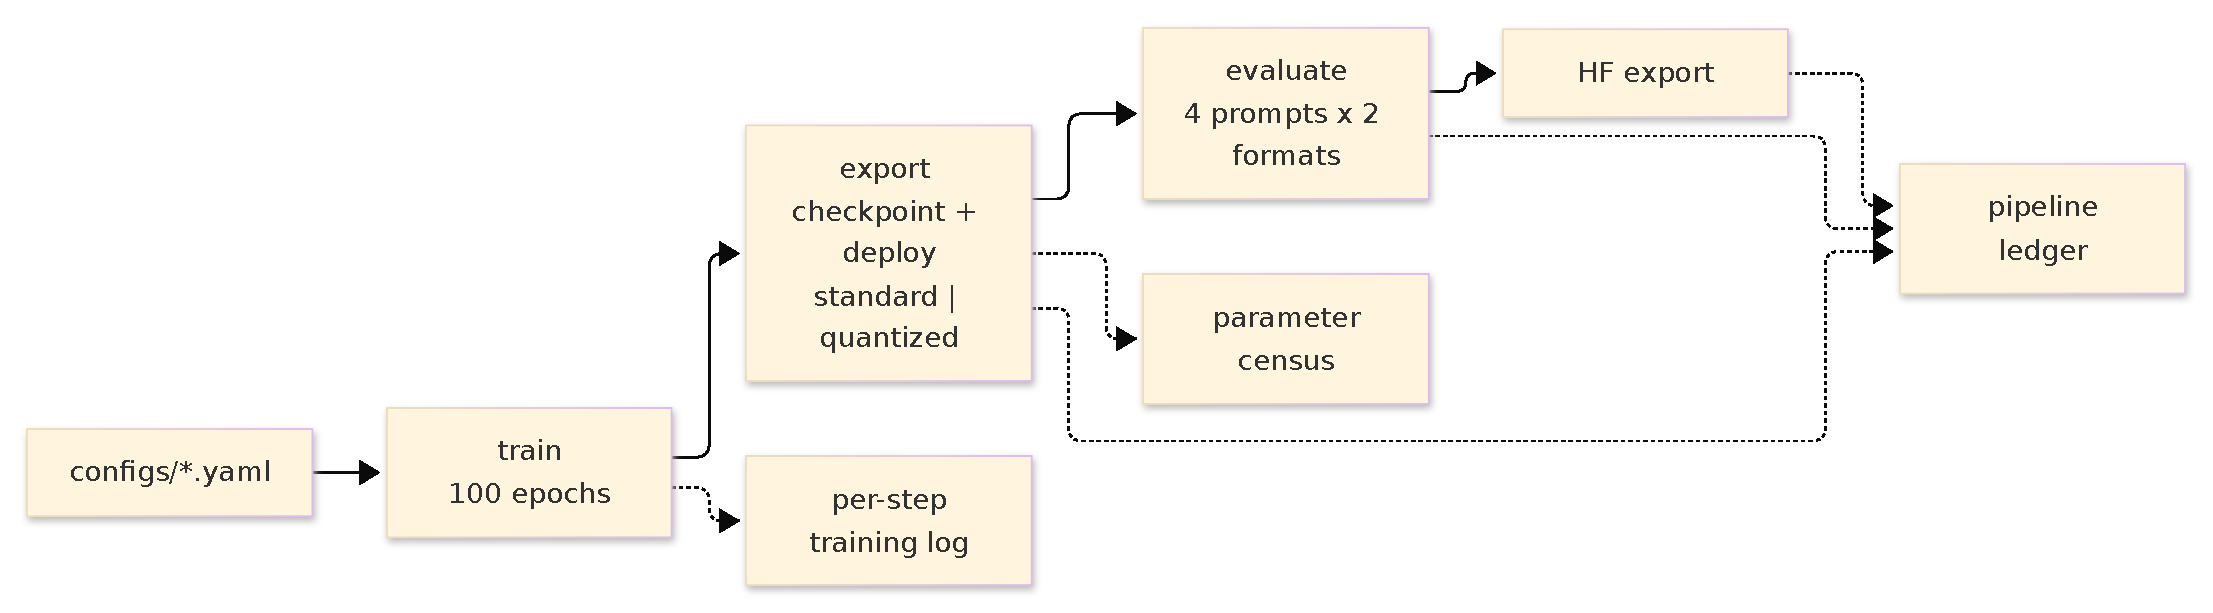
\includegraphics{figures/experiment-pipeline.pdf}}
\caption{One configuration of a round. The five stages are driven by a single YAML file and logged by three independent recorders; the offline reporting toolchain that turns the logs into the published report is documented in Appendix~\ref{sec:annex-experiment-harness}.}
\label{fig:experiment-pipeline}
\end{figure}

Round~2 was generated programmatically. Hybrid pairs are the combinations of the 42-entry mixer list taken two at a time, materialised as a two-layer model whose layer~0 runs mixer~A and layer~1 runs mixer~B; singles use one layer. Because combinations follow the fixed list order, no reversed pair $(B, A)$ exists, so the ``first versus second mixer'' asymmetry reported below is confounded with list order and must be read descriptively. Table~\ref{tab:round2-families} summarises the population.

\begin{table}[H]
\centering
\small
\caption{Round~2 population. Medians are computed per family; the held-out metric is top-1 for MLM pairs and accuracy for the vision, audio and real-data families.}
\label{tab:round2-families}
\begin{tabular}{lrrrrrr}
\toprule
Family & Configs & Median params & Median loss & Median score & Median tok/s & Median min \\
\midrule
Hybrid pairs      & 703 & 220{,}928 & 9.591 & 4.08\%  & 356 & 75.3 \\
Singles           & 38  & 157{,}584 & 9.762 & 3.57\%  & 366 & 24.8 \\
ViT               & 48  & 315{,}694 & 1.205 & 75.97\% & 23  & 9.4  \\
Optimizers        & 23  & 210{,}752 & 10.404 & 7.76\% & 391 & 21.2 \\
Structural        & 20  & 210{,}752 & 10.397 & 5.71\% & 387 & 21.2 \\
Positional enc.   & 12  & 210{,}752 & 10.381 & 7.76\% & 402 & 21.9 \\
Normalization     & 6   & 210{,}512 & 10.348 & 1.61\% & 407 & 20.7 \\
Real data         & 6   & 247{,}788 & 1.060 & 39.04\% & 392 & 7.6  \\
Task              & 4   & 210{,}752 & 8.603 & 5.90\% & 457 & 19.4 \\
Tokenizer         & 4   & 210{,}752 & 5.978 & 4.37\% & 4{,}202 & 1.1 \\
Batch size        & 2   & 210{,}752 & 10.368 & 5.40\% & 596 & 13.0 \\
BitNet/GGUF       & 1   & 209{,}856 & 10.369 & ---    & 562 & ---  \\
Audio             & 1   & 147{,}171 & 1.099 & 0.00\%  & 31{,}082 & 1.2 \\
\bottomrule
\end{tabular}
\end{table}

\subsection{Findings}

\textbf{The second mixer is the stronger lever.} Across the hybrid pairs, the second mixer moves the mean final loss from 9.37 nats (\texttt{sparsek}) to 10.18 (\texttt{mamba}), a spread of 0.81 nats, while the first mixer spans only 0.55 (9.26--9.81 nats, restricted to families with enough samples). Reading the atlas column by column, a good B keeps almost every A in the 8.9--9.6 nat band; reading it row by row, no first mixer rescues a bad second one. At this scale the choice of B dominates the choice of A by about 1.5$\times$.

\textbf{Pairing is not additive.} Defining the synergy of a pair as the average of its two marginal means minus its measured loss, $S_{A,B} = (\mu_A + \mu_B)/2 - L_{A,B}$, the best interaction is \texttt{nsa+engram} at $+1.304$ nats and the worst is \texttt{gqa+tucker} at $-1.018$. The positive tail pairs a cheap, stable first mixer with a memory-heavy second one; the negative tail is dominated by second mixers that look average in isolation (\texttt{gta}, \texttt{gqa}, \texttt{tucker}) but clash when stacked after a strong A. Interaction noise ($\pm 0.3$ nats) is larger than the difference between most optimizers in the ablation.

\textbf{Scale is a weak lever at this size.} Over the hybrid pairs, parameter count correlates with final loss at $r = -0.20$ and with held-out accuracy at $r = -0.07$, while it predicts cost reliably ($r = 0.68$ with step time, $r = 0.65$ with wall-clock). The largest model (\texttt{engram\_\_conformer\_attn}, 415{,}904 parameters) is not the best. Across all 868 rows the correlation appears stronger ($r = -0.43$ for loss), but that is a family confound: vision transformers are both larger and far easier to fit, so the comparison of interest is the within-pairs one.

\textbf{Post-training quantization is essentially free.} Of the 810 configurations deployed in both formats, 800 keep an identical top-5 hit rate; the mean top-1 moves from 5.62\% to 5.43\% and the mean top-5 from 13.36\% to 13.24\%, both deltas within one evaluation sample. Quantized deployment is \emph{not} faster end-to-end (32.3\% of runs, median ratio 0.64$\times$) because the stage is dominated by serialisation and conversion; evaluation itself is faster in 51.2\% of runs with a median 1.03$\times$.

\textbf{The sweep is honest about its failures and its blind spots.} The ledger holds 5{,}271 stage records with 275 failures (171 training, 104 deployment), all outside the 868 analysed configurations. Four mixers (\texttt{cca}, \texttt{ccgqa}, \texttt{msa}, \texttt{ssog}) never train, which accounts exactly for the 158 missing cells of the 861-cell atlas. Four others (\texttt{standard}, \texttt{bigbird}, \texttt{longformer}, \texttt{titan}) produce bit-identical losses because their windows (at least 64 tokens) cover the whole 32-token sequence; the atlas measures one model four times. Separately, 37 pairs appear under both the \texttt{retnet} and \texttt{retnet\_attn} spellings with identical metrics, a duplicate implementation that the analysis collapses.

\textbf{The vision block works.} Segmentation reaches 90.7\% mean held-out accuracy, classification 75.8\% and patch prediction 69.9\%, an order of magnitude above the MLM pairs. That gap reflects task difficulty, not mixer quality, which is why the families are kept separate throughout.

\subsection{Threats to Validity}

The model is small (127k--416k parameters, a 512-token Spanish vocabulary, 32-token sequences, one seed per configuration and 100 epochs). Every learning curve is still descending at epoch~100, so the ranking rewards fast learners rather than converged quality. Inference uses four sentences per configuration, so a single extra hit moves a top-5 rate by 25 percentage points; the held-out signal is a smoke detector for catastrophic failures, not a ranking instrument. Several optimizers converge to the same loss because the run is too short to separate them, and one text-classification run collapsed to a constant prediction, which is a failure mode and not a good model. The rankings in Appendix~\ref{sec:annex-experiment-2} are therefore directional. The next round should re-run the atlas at 256--512 tokens, with a 200-sentence evaluation set, at least three seeds, and 300 epochs for the top pairs.
